\documentclass{article}

\usepackage[tmargin=.9in, bmargin=.9in, lmargin=1in, rmargin=1in]{geometry}
\usepackage{bookmark, wrapfig, enumitem, pdflscape, hyphenat}
\usepackage[labelfont=bf]{caption}
\usepackage{lmodern}
\usepackage[sfdefault]{roboto}
\usepackage[T1]{fontenc}
\usepackage{setspace}

\usepackage{graphicx}
    \makeatletter % tex.stackexchange.com/a/28565
    \setlength{\@fptop}{0pt}
    \setlength{\@fpbot}{0pt plus 1fil}
    \makeatother

\usepackage[absolute, overlay]{textpos}
    \setlength{\TPHorizModule}{1mm}
    \setlength{\TPVertModule}{1mm}

\usepackage{xcolor}
    \definecolor{WCM}{RGB}{172,31,44} % AC1E2C

\usepackage{hyperref} \hypersetup{
    colorlinks=true, linkcolor={blue!65!black},
    citecolor={blue!65!black}, urlcolor={blue!50!black},
    pdfpagelayout=OneColumn, pdfstartview={XYZ null null 1.25},
    bookmarksnumbered=true, bookmarksopen=true, bookmarksopenlevel=3
}

\usepackage[backend=bibtex, style=authoryear]{biblatex}
    \addbibresource{references.bib}
    % https://tex.stackexchange.com/a/134065 :
    \renewcommand*{\nameyeardelim}{\addcomma\space}
    % https://tex.stackexchange.com/a/404787 :
    \usepackage{xpatch}
    \DeclareNameAlias{sortname}{last-first} % general changes
    \renewcommand*{\bibinitdelim}{}
    \renewbibmacro*{in:}{\iffieldequalstr{entrytype}{inproceedings}{\printtext{\bibstring{in}\addspace}}{}}
    \csletcs{abx@macro@publisher+location+date@orig}{abx@macro@publisher+location+date} % changes for "book"
    \renewbibmacro*{publisher+location+date}{\printtext[parens]{\usebibmacro{publisher+location+date@orig}}}
    \DeclareFieldFormat[book]{title}{#1\printunit{\addspace}}
    \DeclareFieldFormat[inproceedings]{title}{#1\isdot} % changes for "inproceedings"
    \DeclareFieldFormat{booktitle}{#1\addcomma}
    \xpatchbibmacro{byeditor+others}
        {\usebibmacro{byeditor+othersstrg} \setunit{\addspace} \printnames[byeditor]{editor} \clearname{editor}}
        {\printnames[byeditor]{editor} \clearname{editor} \addcomma\addspace \bibstring{editor} \setunit{\addspace}}{}{}
    \DeclareFieldFormat[article]{title}{#1} % changes in "article"
    \DeclareFieldFormat[article]{journaltitle}{#1\isdot}
    \DeclareFieldFormat[article]{volume}{\textit{#1}}
    \DeclareFieldFormat[article]{pages}{#1}
    % https://en.wikibooks.org/wiki/LaTeX/Macros#New_commands
    \newcommand{\citep}[1]{(\cite{#1})}

\newcommand{\beginsupplement}{
% bytesizebio.net/2013/03/11/adding-supplementary-tables-and-figures-in-latex
    %\newpage
    %\setcounter{page}{1}
    %\renewcommand{\thepage}{S-\arabic{page}}
    \pagenumbering{gobble}
    \setcounter{table}{0}
    \renewcommand{\thetable}{S\arabic{table}}
    \setcounter{figure}{0}
    \renewcommand{\thefigure}{S\arabic{figure}}
 }
\begin{document}

\beginsupplement

\section*{Supplemental Information}

\subsection*{Supplemental figures} \addcontentsline{toc}{subsection}{Supplemental figures} \label{sec:supp_figs}

\begin{figure}[ht!] \centering
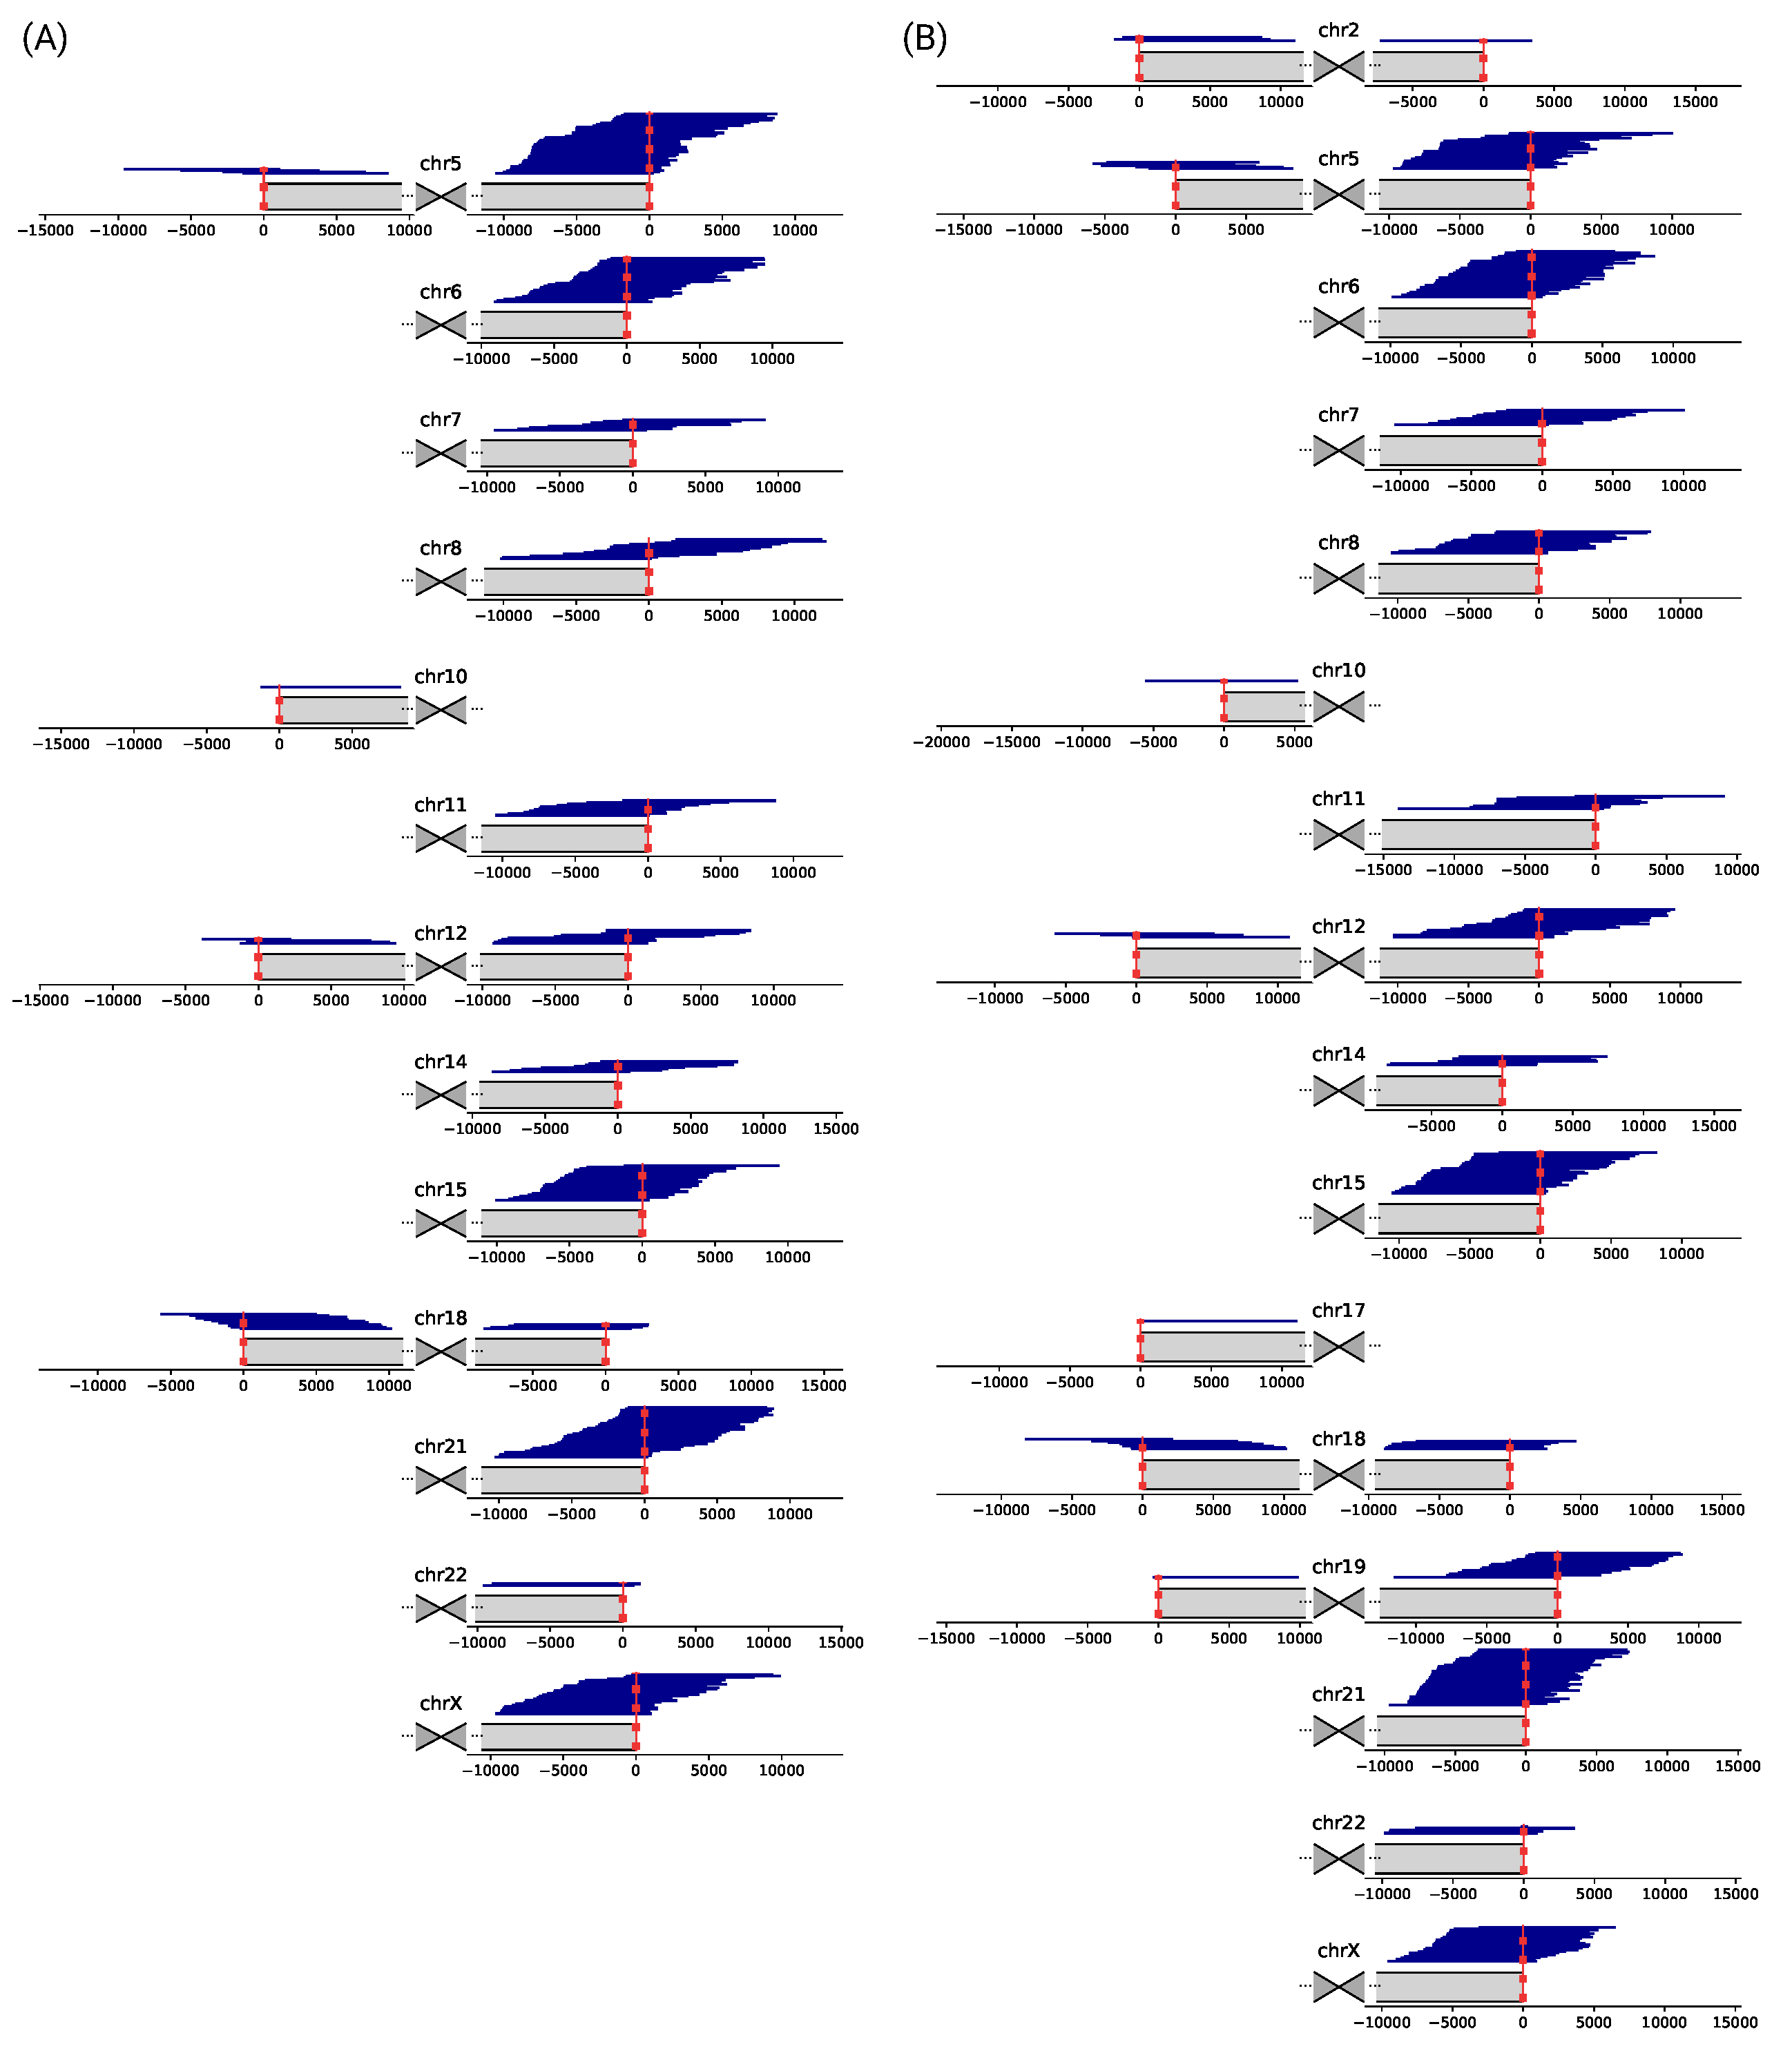
\includegraphics[height=.65\textheight,width=\textwidth,keepaspectratio]{figures/HG00X-alignments.pdf}
\caption{
    Mapping of candidate telomeric PacBio CCS reads from datasets (A) HG001 and (B) HG005.
    Chromosomes are displayed schematically, centered around the centromere, with only the arms shown to which candidate reads aligned.
    Vertical red dashed lines denote the position of the boundary of the annotated telomeric tract.
    Coordinates are given in bp, relative to the positions of the telomeric tract boundaries.
    Relates to: \textbf{Figure 1}.
}
\label{fig:hg00x_alignments}
\end{figure}
\clearpage \pagebreak

\begin{figure}[ht!] \centering
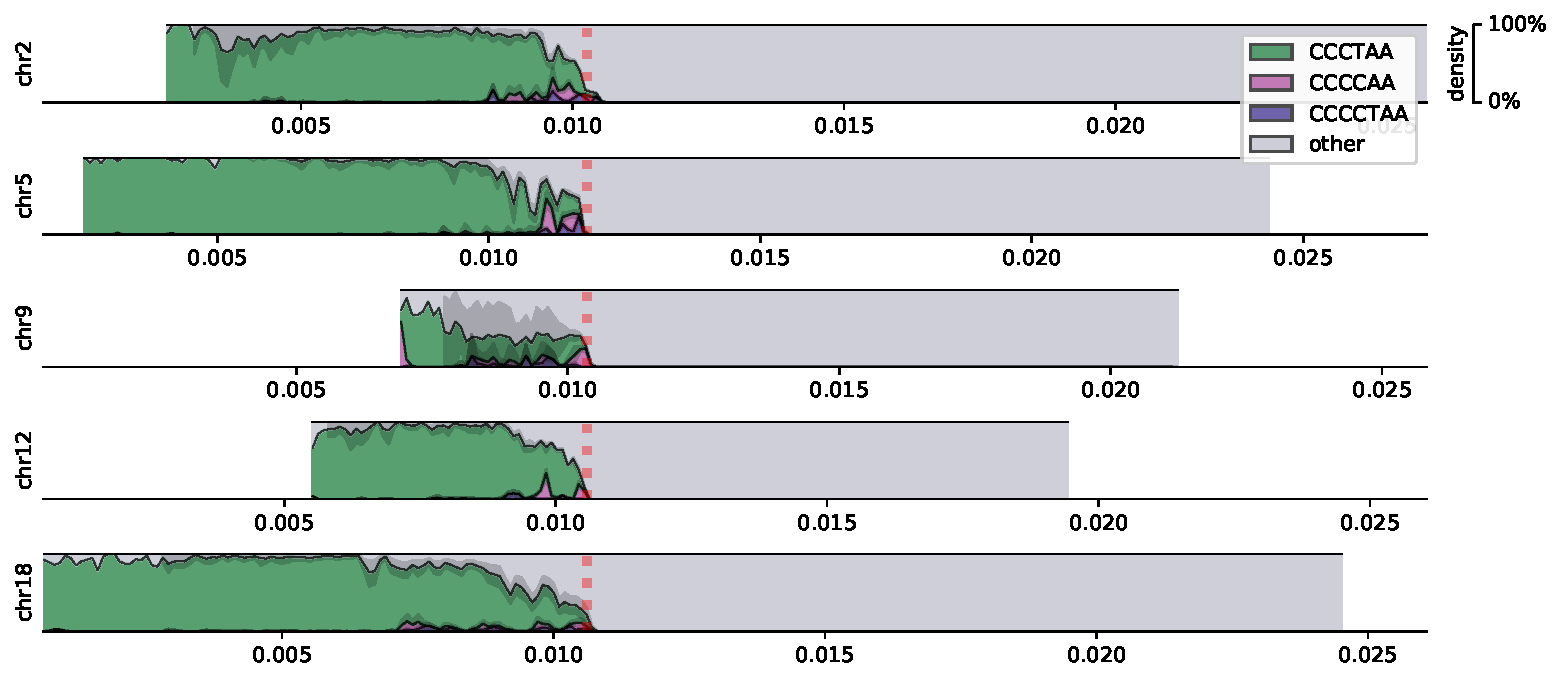
\includegraphics[height=.9\textheight,width=\textwidth,keepaspectratio]{figures/threemotifp/HG002-densityplot-p_arm-threemotifp.pdf}
\caption{
    Densities of top three enriched motifs (contributing to at least 0.5\% of the repeat content) at ends of chromosomal \textit{p} arms of the HG002 dataset.
    Only the arms covered by at least 20 reads are displayed.
    Genomic coordinates are given in Mbp.
    Vertical red dashed lines denote the position of the boundary of the annotated telomeric tract.
    Relates to: \textbf{Figure 2}, \textbf{Table 1}.
}
\label{fig:hg002_densityplot_p_arm}
\end{figure}
\clearpage \pagebreak

\begin{figure}[ht!] \centering
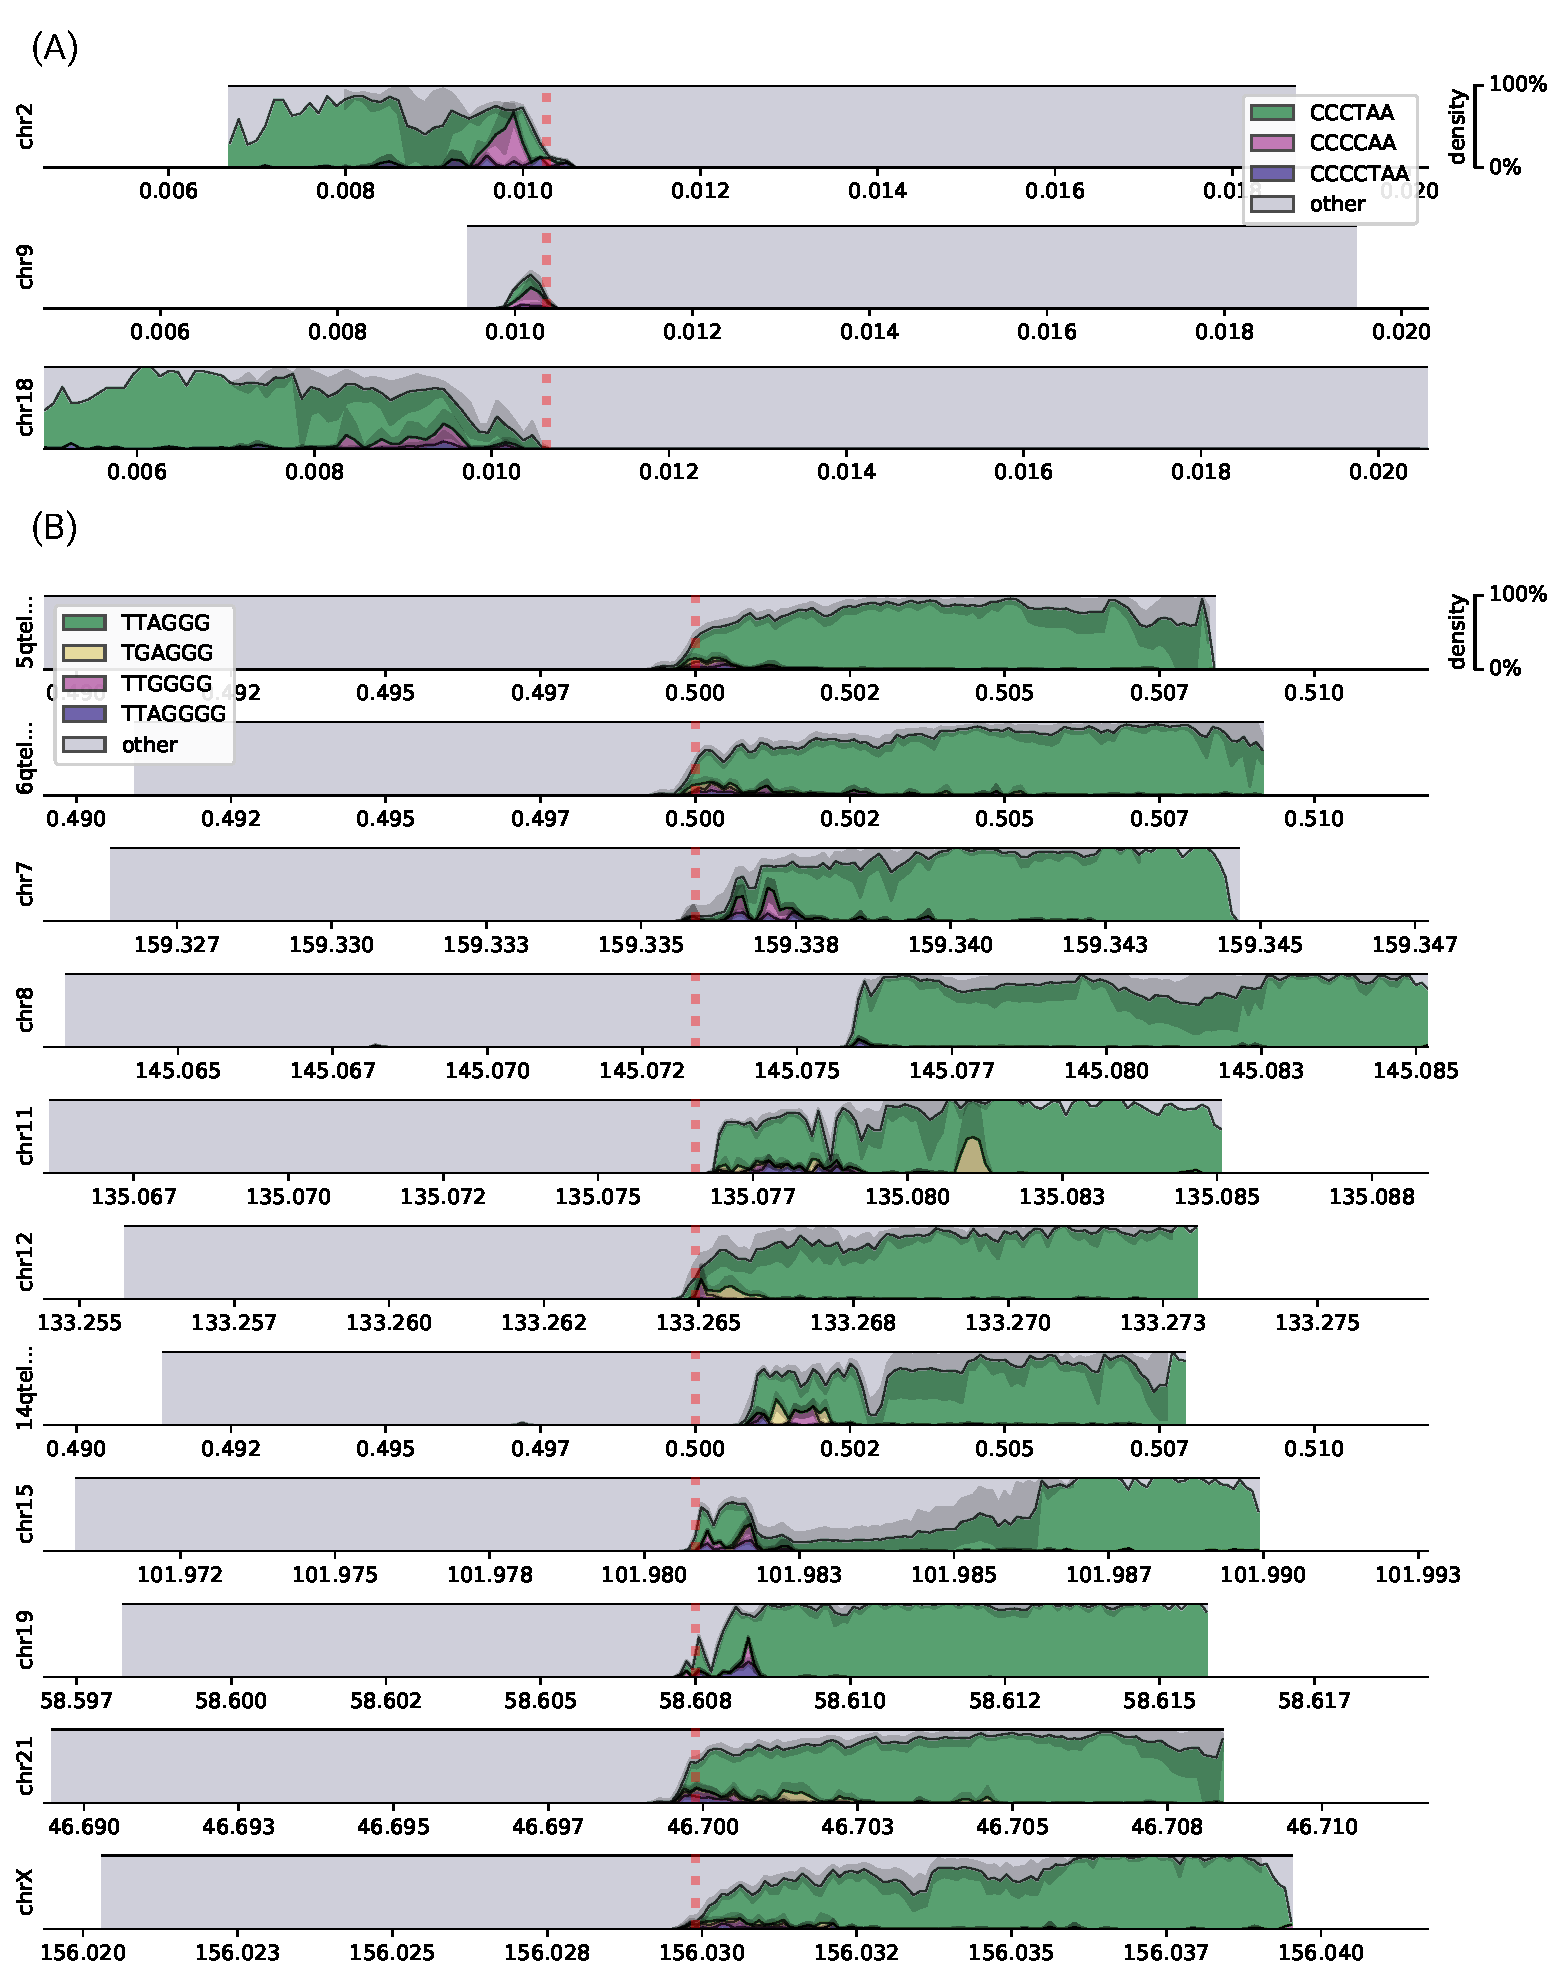
\includegraphics[height=.95\textheight,width=\textwidth,keepaspectratio]{figures/threemotifp/HG001-densityplots-threemotifp.pdf}
\caption{
    Motif densities at ends of chromosomal (A) \textit{p} and (B) \textit{q} arms of the HG001 dataset.
    Only the arms covered by at least 20 reads are displayed.
    Genomic coordinates are given in Mbp.
    Relates to: \textbf{Figure 2}, \textbf{Table 1}.
}
\label{fig:hg001_densityplots}
\end{figure}
\clearpage \pagebreak

\begin{figure}[ht!] \centering
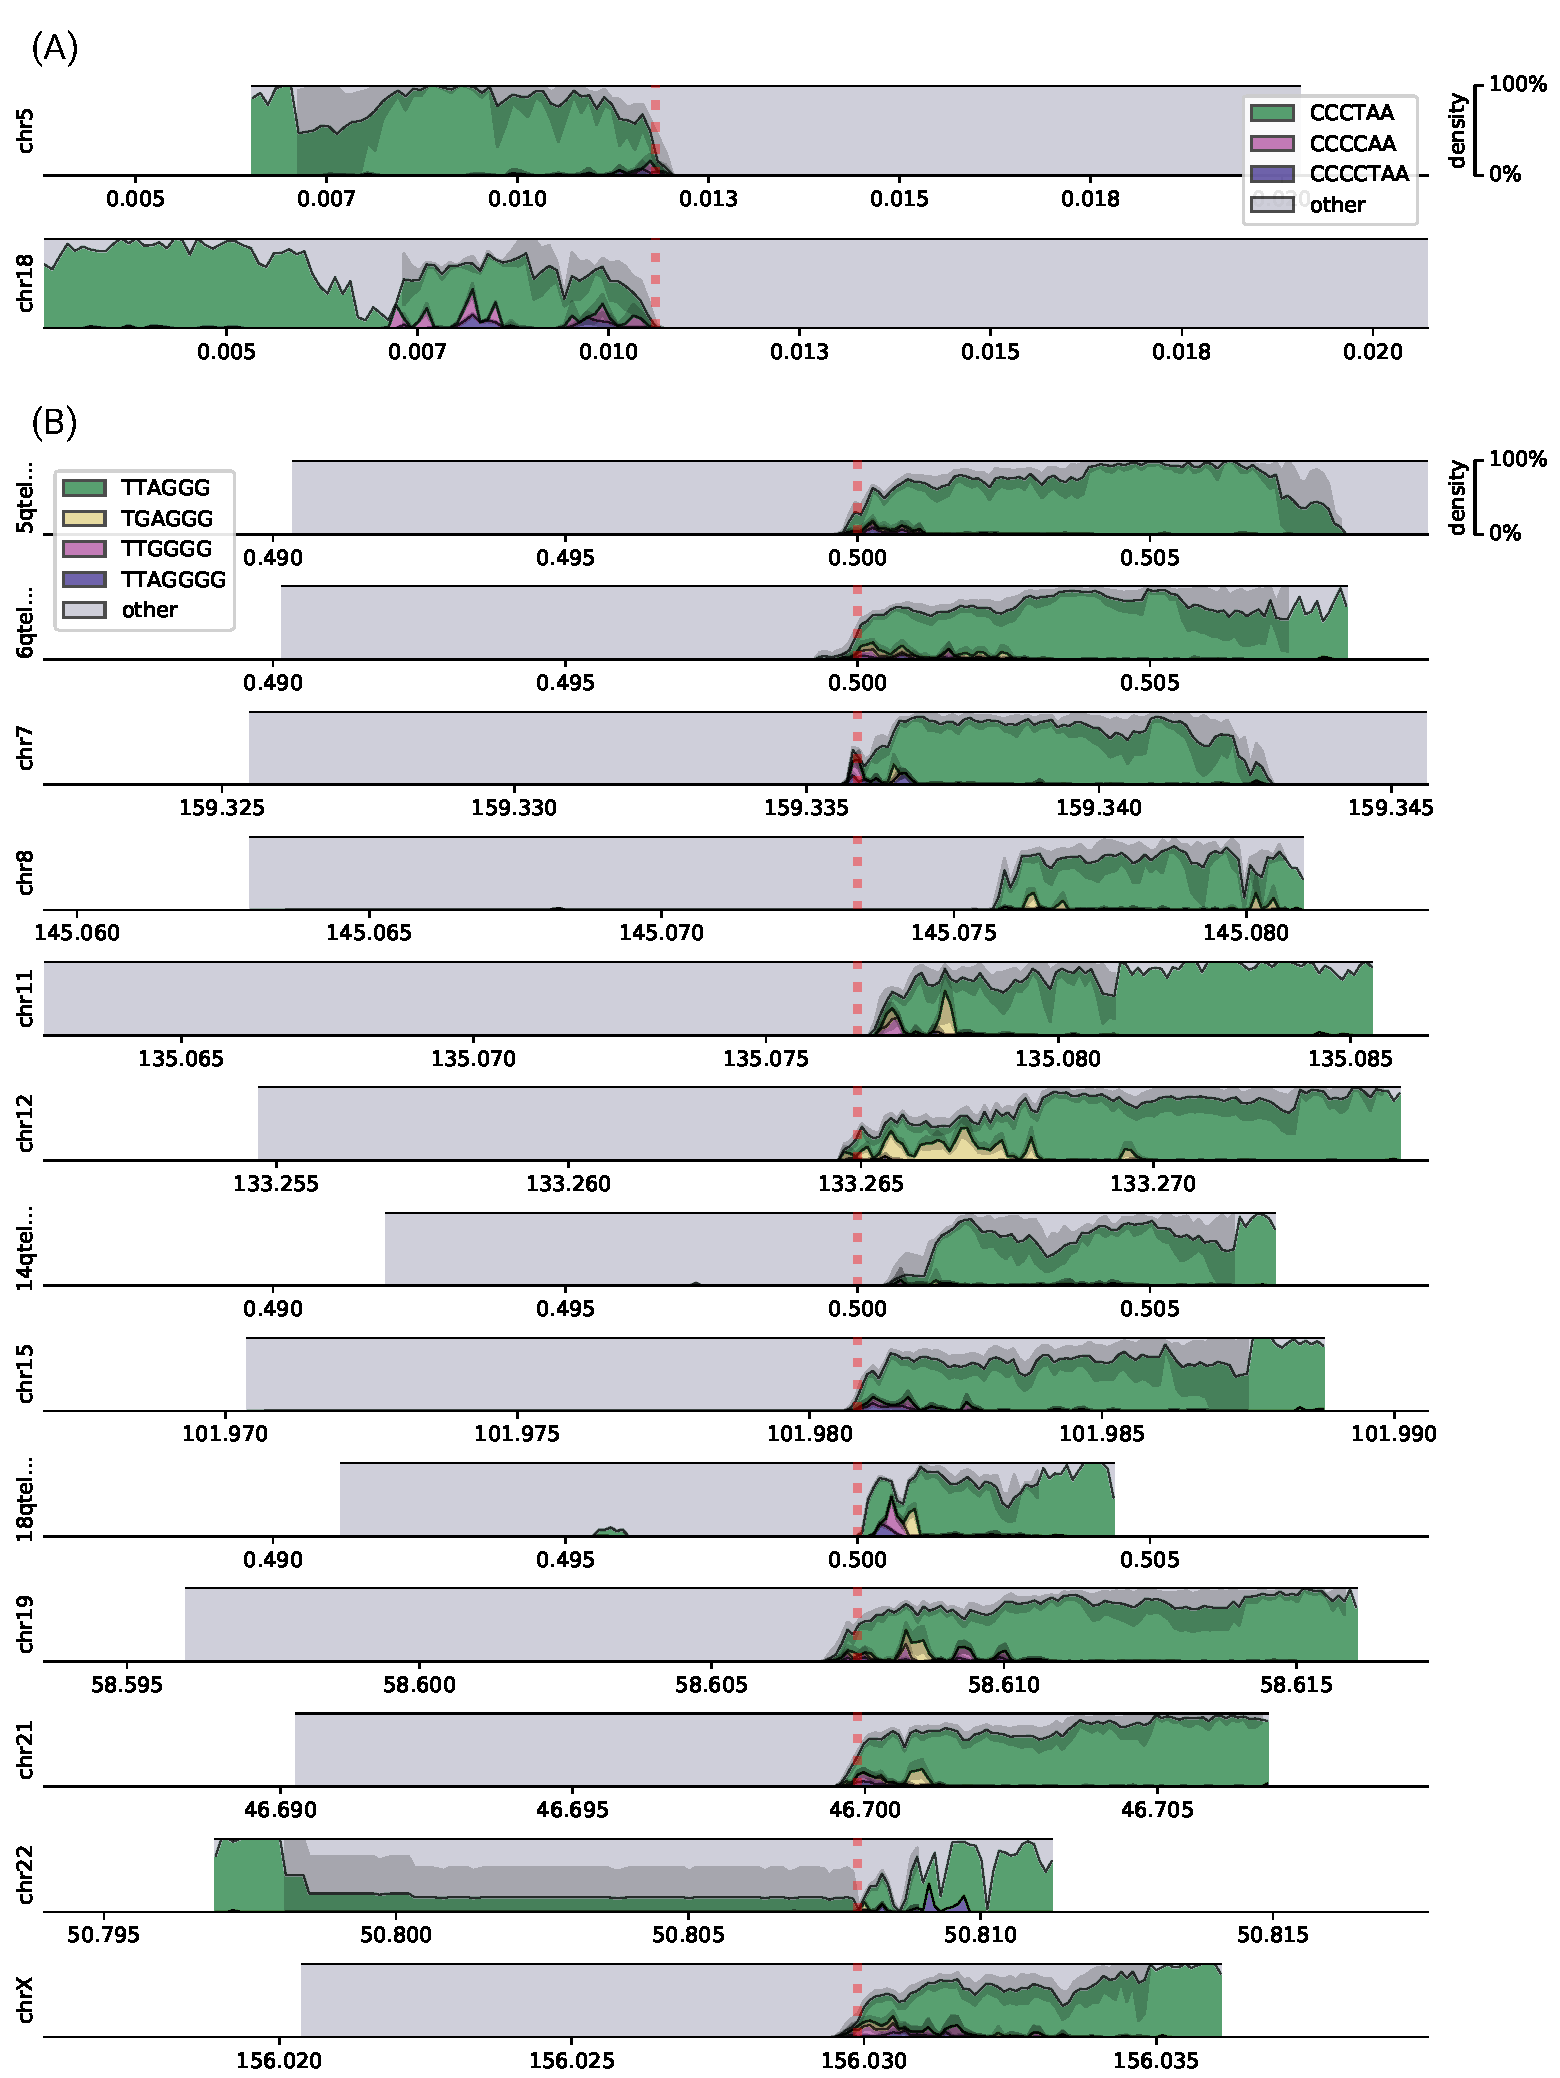
\includegraphics[height=.95\textheight,width=\textwidth,keepaspectratio]{figures/threemotifp/HG005-densityplots-threemotifp.pdf}
\caption{
    Motif densities at ends of chromosomal (A) \textit{p} and (B) \textit{q} arms of the HG005 dataset.
    Only the arms covered by at least 20 reads are displayed.
    Genomic coordinates are given in Mbp.
    Relates to: \textbf{Figure 2}, \textbf{Table 1}.
}
\label{fig:hg005_densityplots}
\end{figure}
\clearpage \pagebreak

\begin{figure}[ht!] \centering
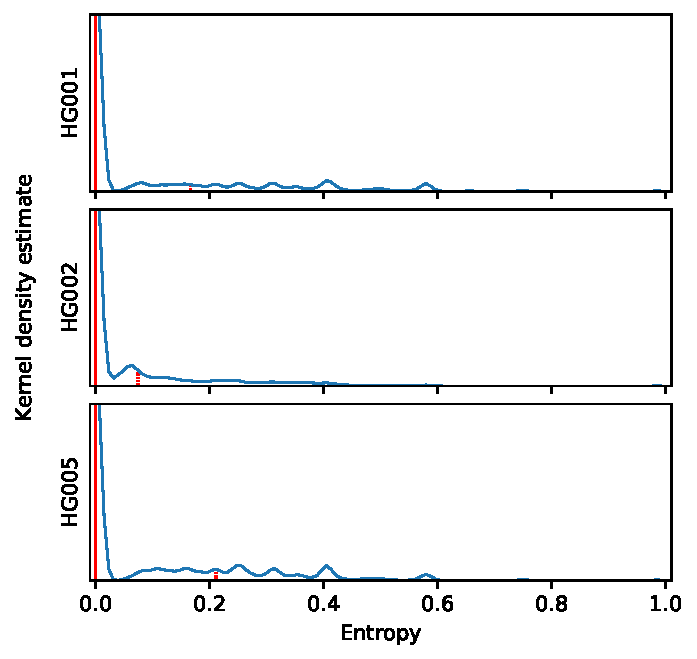
\includegraphics[height=.95\textheight,width=.65\textwidth,keepaspectratio]{figures/entropy.pdf}
\caption{
    Distribution of motif entropies in 10 bp windows of candidate PacBio CCS reads aligning to the same chromosomal arms in GIAB datasets HG001, HG002, and HG005.
    Red solid lines denote the position of the median (0.000 in all three datasets), and red dashed lines denote the 3rd quartile (0.166, 0.074, and 0.211, respectively).
    Relates to: \textbf{STAR Methods, Evaluation of sequence concordance in telomeric long reads}.
}
\label{fig:entropy}
\end{figure}
\clearpage \pagebreak

\subsection*{Supplemental tables} \addcontentsline{toc}{subsection}{Supplemental tables}
\begin{samepage} \begin{table}[h!] \begin{tabular}{llllll}
\hline
\textbf{chromosome}  &  \textbf{reference contig}        &  \textbf{arm}  &  \textbf{HG001}  &  \textbf{HG002}  &  \textbf{HG005} \\
\hline
chr2                 &  2qtel\_1-500K\_1\_12\_12\_rc     &  q             &  0               &  0               &  1              \\
chr2                 &  chr2                             &  p             &  5               &  16              &  3              \\
chr5                 &  5qtel\_1-500K\_1\_12\_12\_rc     &  q             &  42              &  53              &  23             \\
chr5                 &  chr5                             &  p             &  4               &  15              &  5              \\
chr6                 &  6qtel\_1-500K\_1\_12\_12\_rc     &  q             &  31              &  49              &  29             \\
chr7                 &  chr7                             &  q             &  8               &  32              &  10             \\
chr8                 &  chr8                             &  q             &  14              &  35              &  14             \\
chr9                 &  chr9                             &  p             &  6               &  6               &  0              \\
chr10                &  10qtel\_1-500K\_1\_12\_12\_rc    &  q             &  0               &  1               &  0              \\
chr10                &  chr10                            &  p             &  1               &  2               &  1              \\
chr11                &  chr11                            &  q             &  11              &  31              &  9              \\
chr12                &  chr12                            &  q             &  10              &  27              &  18             \\
chr12                &  chr12                            &  p             &  4               &  5               &  3              \\
chr14                &  14qtel\_1-500K\_1\_12\_12\_rc    &  q             &  8               &  26              &  6              \\
chr15                &  chr15                            &  q             &  25              &  21              &  26             \\
chr16                &  16qtel\_1-500K\_1\_12\_12\_rc    &  q             &  0               &  2               &  0              \\
chr16                &  chr16                            &  p             &  1               &  0               &  0              \\
chr17                &  17qtel\_1-500K\_1\_12\_12v2\_rc  &  q             &  0               &  4               &  0              \\
chr17                &  17ptel\_1\_500K\_1\_12\_12       &  p             &  0               &  1               &  1              \\
chr18                &  18qtel\_1-500K\_1\_12\_12\_rc    &  q             &  4               &  26              &  6              \\
chr18                &  chr18                            &  p             &  11              &  35              &  7              \\
chr19                &  19ptel\_1-500K\_1\_12\_12        &  p             &  0               &  1               &  1              \\
chr19                &  chr19                            &  q             &  6               &  0               &  16             \\
chr21                &  chr21                            &  q             &  35              &  77              &  35             \\
chr22                &  chr22                            &  q             &  2               &  51              &  5              \\
chrX                 &  chrX                             &  q             &  28              &  54              &  22             \\
\hline
\end{tabular}
\caption{The number of telomeric reads on each arm identified in GIAB PacBio CCS datasets HG001, HG002, and HG005.}
\label{tab:telomeric_read_counts}
\end{table}
\end{samepage}

\begin{samepage} \begin{table}[h!] \small \begin{tabular}{lllll}
\hline
\textbf{Motif}  & \multicolumn{2}{l}{\textbf{Illumina datasets}}        & \multicolumn{2}{l}{\textbf{10X datasets}}             \\
\textbf{}       & \textbf{Median abundance} & \textbf{Adjusted p-value} & \textbf{Median abundance} & \textbf{Adjusted p-value} \\
\hline
TTAGGG          & 0.299068                  & 0.00e+0                   & 0.461711              & 0.00e+0                       \\
TGAGGG          & 0.007484                  & 0.00e+0                   & 0.018524              & 0.00e+0                       \\
TTGGGG          & 0.002495                  & 0.00e+0                   & 0.007190              & 0.00e+0                       \\
GGGG            & 0.020347                  & 0.00e+0                   & 0.006080              & 0.00e+0                       \\
TTAGGGG         & 0.003007                  & 0.00e+0                   & 0.005024              & 0.00e+0                       \\
TTTT            & 0.001294                  & 0.00e+0                   & 0.001490              & 0.00e+0                       \\
TTAAGGG         & 0.000664                  & 1.39e-55                  & 0.001124              & 1.58e-59                      \\
TTAGGGGTTAGGG   & 0.000533                  & 1.04e-51                  & 0.001020              & 0.00e+0                       \\
TAGGG           & 0.000619                  & 0.00e+0                   & 0.001020              & 0.00e+0                       \\
TTGGG           & 0.000500                  & 0.00e+0                   & 0.000989              & 0.00e+0                       \\
TTTAGGG         & 0.000622                  & 6.40e-55                  & 0.000884              & 1.02e-57                      \\
TAGGGTTAGGG     & 0.000312                  & 4.24e-40                  & 0.000503              & 0.00e+0                       \\
TTAGGGTTTAGGG   & 0.000176                  & 4.41e-38                  & 0.000284              & 6.22e-59                      \\
TTAGGGTTAAGGG   & 0.000145                  & 6.63e-36                  & 0.000264              & 4.15e-57                      \\
TTAGG           & 0.000241                  & 8.13e-35                  & 0.000213              & 1.10e-55                      \\
TTGGGTTAGGG     & 0.000127                  & 4.47e-28                  & 0.000178              & 3.34e-56                      \\
TTAGGGTTAGG     & 0.000066                  & 1.99e-18                  & 0.000092              & 7.82e-48                      \\
TTAGGGGG        & 0.000039                  & 1.02e-14                  & 0.000062              & 4.31e-40                      \\
TTAGGGTTGTTAGGG & 0.000035                  & 4.64e-09                  & 0.000061              & 4.65e-57                      \\
TTAGAGGG        & 0.000036                  & 5.44e-13                  & 0.000053              & 2.66e-36                      \\
TTGGGGTTGGGGG   & 0.000002                  & 4.51e-13                  & 0.000014              & 5.84e-21                      \\
TTAGGGTGGTTAGGG & 0.000007                  & 5.39e-06                  & 0.000013              & 5.42e-38                      \\
\hline
\end{tabular}
\caption{Significantly enriched repeating motifs in telomeric candidate reads in short-read sequencing experiments, subset to motifs also observed in PacBio telomeric reads, with respect to reverse-complement equivalence. Relates to: \textbf{STAR Methods, Identification of repeat content}.}
\label{tab:shortread_repeatfinder}
\end{table}
\end{samepage}

\begin{samepage} \begin{table}[h!] \begin{tabular}{llll}
\hline
\textbf{Chromosome}            &  \textbf{Haplotype}  &  \textbf{PacBio\_CCS\_10kb}  &  \textbf{PacBio\_CCS\_15kb}  \\
\hline
5qtel\_1-500K\_1\_12\_12\_rc   &  1                   &  11                          &  24                          \\
5qtel\_1-500K\_1\_12\_12\_rc   &  2                   &  7                           &  10                          \\
6qtel\_1-500K\_1\_12\_12\_rc   &  1                   &  8                           &  12                          \\
6qtel\_1-500K\_1\_12\_12\_rc   &  2                   &  18                          &  10                          \\
chr7                           &  1                   &  9                           &  8                           \\
chr7                           &  2                   &  7                           &  8                           \\
chr8                           &  1                   &  8                           &  6                           \\
chr8                           &  2                   &  9                           &  8                           \\
chr11                          &  1                   &  5                           &  11                          \\
chr11                          &  2                   &  8                           &  7                           \\
chr12                          &  1                   &  9                           &  9                           \\
chr12                          &  2                   &  6                           &  3                           \\
14qtel\_1-500K\_1\_12\_12\_rc  &  1                   &  3                           &  8                           \\
14qtel\_1-500K\_1\_12\_12\_rc  &  2                   &  5                           &  10                          \\
chr15                          &  1                   &  6                           &  0                           \\
chr15                          &  2                   &  4                           &  11                          \\
18qtel\_1-500K\_1\_12\_12\_rc  &  1                   &  4                           &  9                           \\
18qtel\_1-500K\_1\_12\_12\_rc  &  2                   &  4                           &  9                           \\
chr21                          &  1                   &  16                          &  20                          \\
chr21                          &  2                   &  12                          &  29                          \\
chr22                          &  1                   &  2                           &  27                          \\
chr22                          &  2                   &  11                          &  10                          \\
chrX                           &  1                   &  12                          &  13                          \\
chrX                           &  2                   &  10                          &  19                          \\
\hline
\end{tabular}
\caption{Amounts of reads from the two HG002 PacBio CCS sequencing experiments contributing to each telomeric haplotype on the \textit{q} arms. Relates to: \textbf{Figure 3}.}
\label{tab:hg002_haplotype_assignment}
\end{table}
\end{samepage}


\end{document}
